\section{Limite e Continuidade}

%
%\begin{frame}
%	\frametitle{Noções de Topologia no $\R^2$ }
%	\begin{scriptsize}
%		
%		\uncover<1->{Dados $r>0$ e $P_0=(x_0,y_0)\in \R^2$ o conjunto
%			$$\{(x,y)\in \R^2; (x-x_0)^2+(y-y_0)^2<r\}$$
%			denomina-se \dt{bola aberta} de centro $(x_0,y_0)$ e raio $r>0$ e é denotado por $B_r(P_0)$.
%			\bigskip
%			
%			Seja $U$ um subconjunto de $\R^2$. Dizemos que um ponto $(x_0,y_0)\in U$ é um \dt{ponto interior} de $U$ se existir uma bola aberta de centro em $(x_0,y_0)$ interiamente contida  em $U$.  
%			
%			\begin{exe}Seja $U=\{(x,y)\in\R^2;\ x\geq 0, y\geq 0\}$\begin{enumerate}[a]
%					\item O ponto $(1,2)$ é ponto interior a $U$.
%					\item Todo ponto tal que $(x,y)$ tal que $x>0$ e $y>0$ é ponto interiro a $U$.
%					\item $(0,1)$ não é ponto interior a $U$
%				\end{enumerate}
%			\end{exe}
%			
%		}
%		
%	\end{scriptsize}
%\end{frame}
%
%
%\begin{frame}
%	\frametitle{ }
%	\begin{scriptsize}
%		
%		\uncover<1->{Dado $U\subset\R^2$, dizemos que um ponto $(x_0,y_0)$ é \dt{ponto de fronteira} de $U$ se para toda bola aberta de centro em $(x_0,y_0)$ contém pontos de $U$ e pontos em $\R^2\setminus U$. O conjunto de todos os pontos de fronteira de $U$ é denominado \dt{fronteira de $U$} e denotado por $\partial U$. 
%			\bigskip
%			
%			Um conjunto $U$ é dito $aberto$ quando todos os seus pontos são pontos interiores. Um conjunto é dito \dt{fechado} contém todos os seus pontos de fronteira..
%			\bigskip
%			
%			Um ponto $(x_0,y_0)\in U$ é dito \dt{ponto de acumulação } de $U$ quando toda bola $B_r(x_0,y_0)$ contém pelo menos um ponto  de $U$ diferente de $U$.
%		}
%		
%		\uncover<2->{\begin{exe} 
%				\begin{enumerate}[a)]
%					\item Toda bola aberta é um conjunto aberto.
%					\item $\R^2$ e o conjunto vazio são conjuntos aberto e fechado ao mesmo tempo.
%					\item $U=\{(x,y)\in \R^2;\ x\geq 0 \mbox{ e } y>0 \}$ não é aberto e nem fechado.
%					\item $(0,0)$ é ponto de acumulação de $U=\{\left(\frac{1}{n},0\right);\ n\in\mathbb{N}\}$.
%				\end{enumerate}
%		\end{exe}}
%		
%	\end{scriptsize}
%\end{frame}

\subsection*{Limites}
\begin{frame}[label=limites]{Limites}
Seja $f:D\subset\R^2\to \R$ uma função cujo domínio contém pontos arbitrariamente próximos de {\color{blue}$(a,b)$}. Usamos a notação 
	\[\lim_{(x,y)\to {\color{blue}(a,b)}}f(x,y)={\color{red}L},\]
	para indicar que os valores de $f(x,y)$ se aproximam do número {\color{red}$L$} quando o ponto $(x,y)$ se aproxima do ponto {\color{blue}$(a,b)$} ao longo de qualquer cominho contido no domínio da função $f$.
\end{frame}

\subsection*{definição}
\begin{frame}[label=limites]
	\frametitle{Limite}
%	\begin{scriptsize}
		
		\begin{defin} Seja $f:D\subset\R^2\to \R$ uma função cujo domínio contém pontos arbitrariamente próximos de {\color{blue}$(a,b)$}. Dizemos que {\color{blue} o limite de $f(x,y)$ quando $(x,y)$ tende a $(a,b)$} é o número {\color{blue}$L$}, e escrevemos
				\[\lim_{(x,y)\to {\color{blue}(a,b)}}f(x,y)={\color{red}L},\]
				quando para cada $\varepsilon>0$, existe $\delta>0$ tal que se $\|(x,y)-{\color{blue}(a,b)}\|<\delta$, então $|f(x,y)-{\color{red}L}|<\varepsilon$.
		\end{defin} 

\end{frame}

\begin{frame}[label=limites]
	\begin{center}
		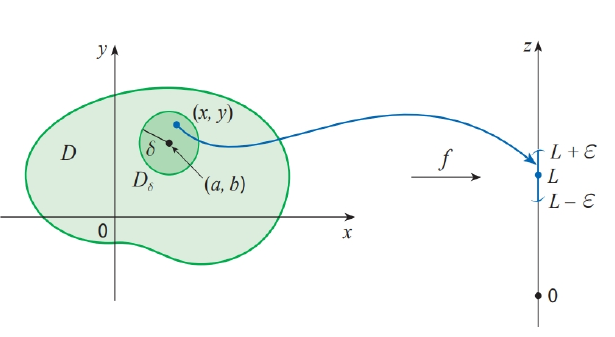
\includegraphics[scale=0.5]{figuras/limite1.png}

		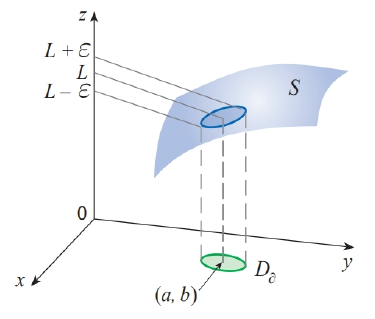
\includegraphics[scale=0.5]{figuras/limite2.png}

	\end{center}
\end{frame}


\begin{frame}[label=limites]
		Todas as propriedades de limites de funções  de uma variável se estendem às funções de várias variáveis. Por exemplo, o limite da soma, diferença, produto ou quociente é a soma, diferença, produto ou quociente dos limites, respectivamente, contanto que esses limites existam e que os denominadores não se anulem.
		\begin{exe} Calcule 
			$\dps\lim_{(x,,y)\to(-1,2)}\left(2x^2y-\frac{3y^2}{x+y}\right).$
	\end{exe}
\end{frame}


\begin{frame}[label=limites]{Mostrando que um limite não existe}

Quando o limite de uma função existe em um ponto, então o limite tem que ser o mesmo ao longo de todos os caminhos que se aproximam do ponto. 
\smallskip 

No plano podemos nos aproximar de um ponto {\color{blue}$(a,b)$} por {\color{red} um número infinito de caminhos}, assim se existem dois caminhos diferentes tais que $f(x,y)$ tende a valores distintos, então o limite não existe.


\begin{center}
	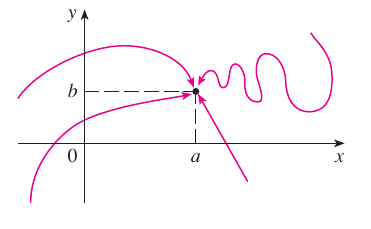
\includegraphics[scale=0.5]{figuras/lim-caminhos.png}
\end{center}

		
\end{frame}

\subsection*{Não existência de limite}
\begin{frame}[label=limites]
	\begin{exe} Mostre que o seguinte limite não existe
		\[\lim_{(x,y)\to(0,0)}\frac{x^2-y^2}{x^2+y^2}.\]
	\end{exe}  

	\begin{center}
		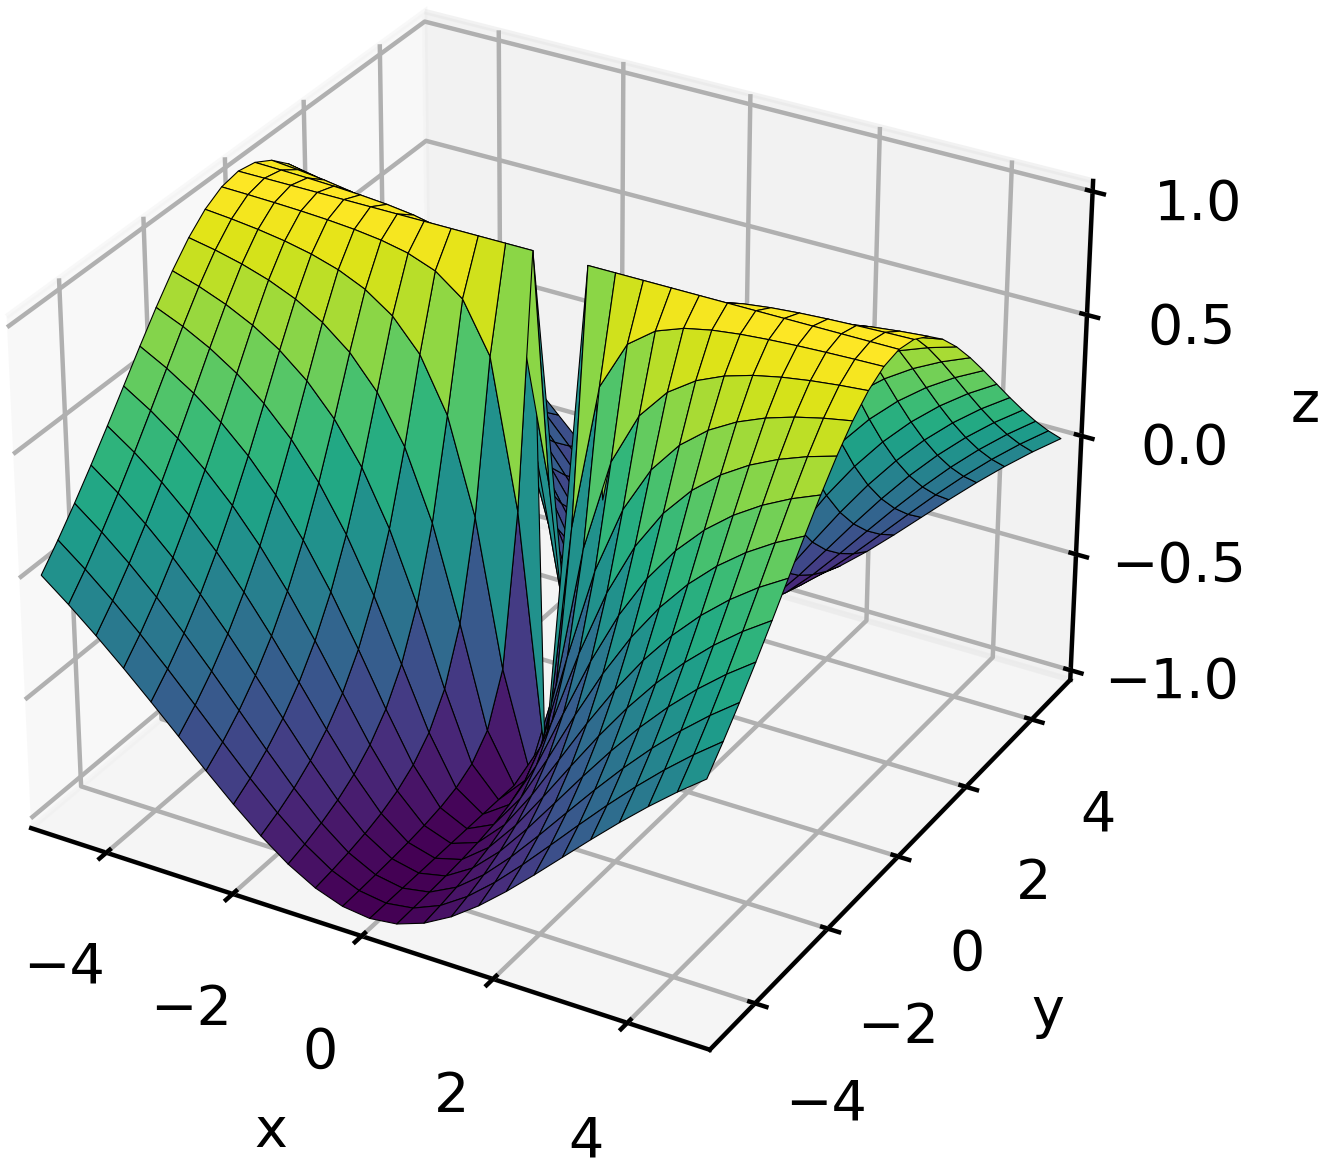
\includegraphics[scale=0.7]{figuras/lim1.png}
	\end{center}

\end{frame}

\begin{frame}[label=limites]
	\begin{exe}
		Mostre que o seguinte limite não existe
		\[\lim_{(x,y)\to(0,0)}\frac{xy}{x^2+y^2}\]
	\end{exe}

	\begin{center}
	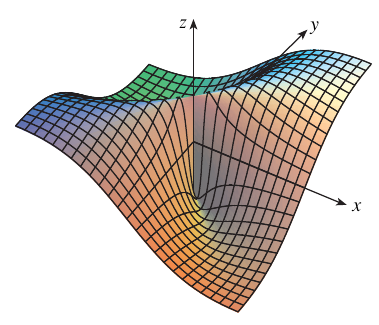
\includegraphics[scale=0.7]{figuras/lim2.png}
\end{center}
\end{frame}

\begin{frame}[label=limites]
	\begin{exe}
		Mostre que o seguinte limite existe
		\[\lim_{(x,y)\to(0,0)}\frac{2x^2y}{x^2+y^2}\]
	\end{exe}
	\begin{center}
	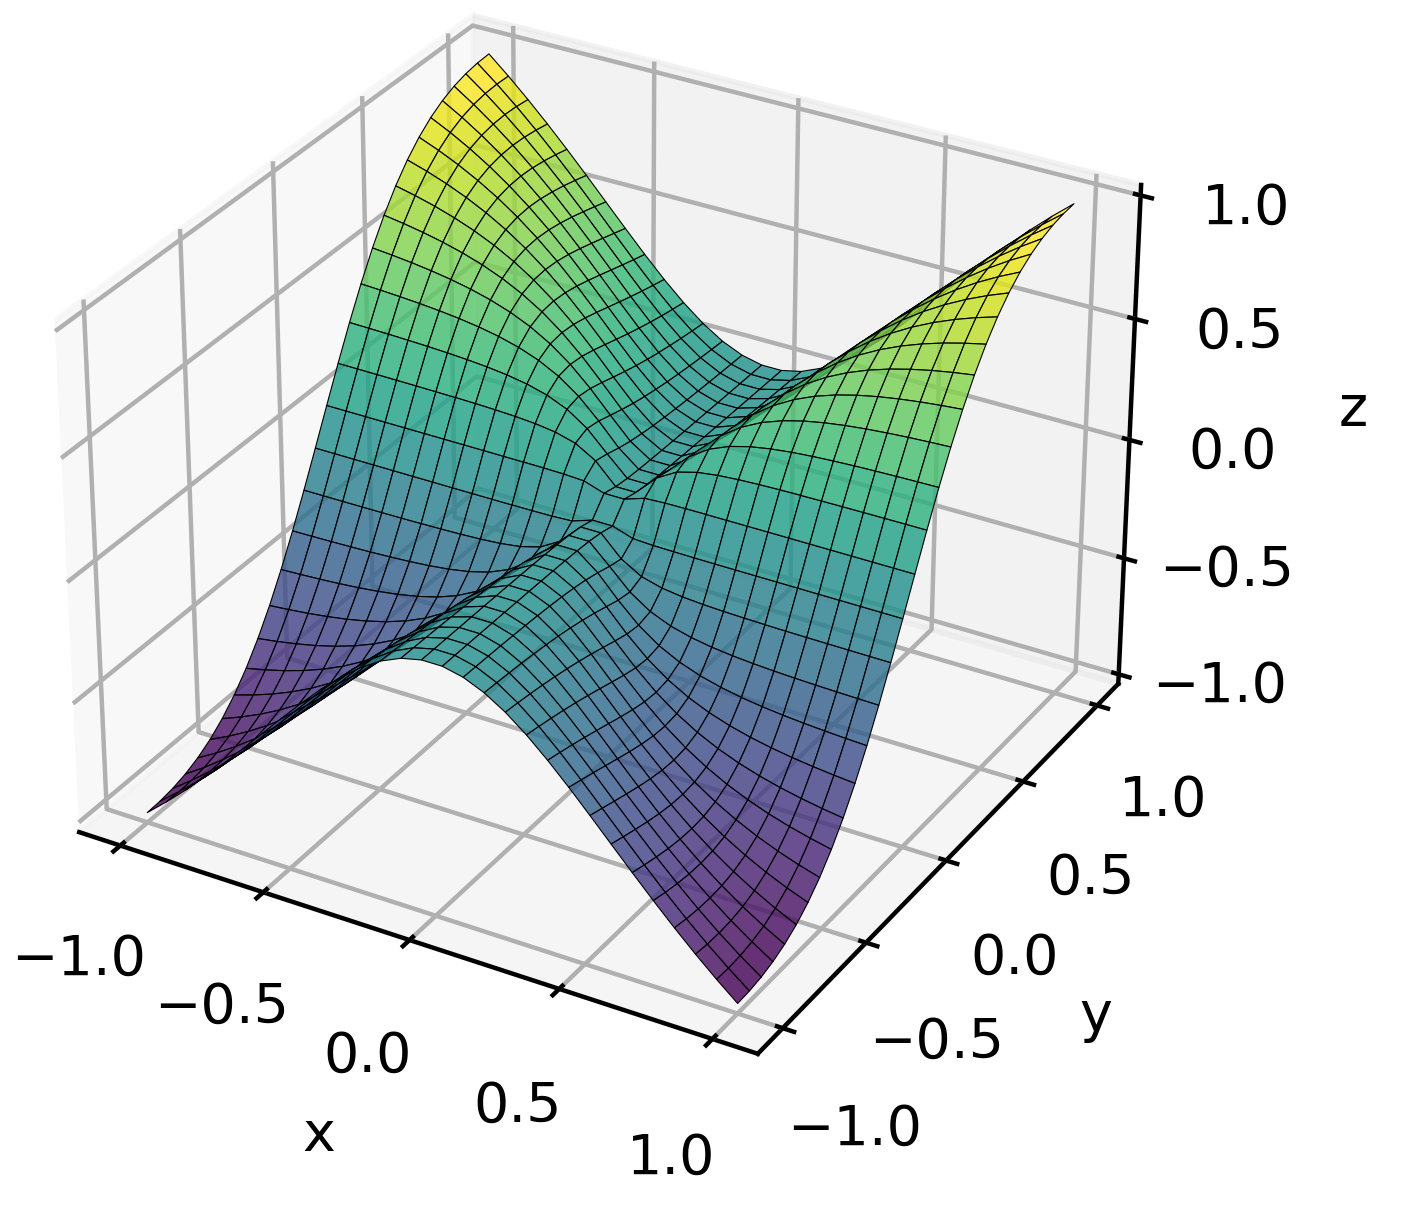
\includegraphics[scale=0.7]{figuras/lim3.png}
\end{center}
\end{frame}

\subsection*{Continuidade}
\begin{frame}[label=limites]
	\frametitle{Continuidade }

		
		\uncover<1->{\begin{defin} Sejam $f$ uma função real de duas variáveis e $(a,b)$ um ponto do domínio de $f$. Dizemos que $f$ é \dt{contínua} em $\pz$ se 
				$$\lim_{(x,y)\to\pz}f(x,y)=f\pz.$$
				Dizemos que $f$ é contínua em $D$ se $f$ é contínua em todos os pontos de $D$.
			\end{defin} 
		 }
		

\end{frame}


\begin{frame}[label=limites]
	
\begin{exe} \begin{enumerate}[a]
		\item Funções racionais são contínuas em todos os pontos de seu domínio.
		
		
		\item  A função $\arctan\left(\frac{y}{x}\right)$ é contínua em todo o seu domínio pois a composta de funções contínuas também é contínua.
	\end{enumerate}
\end{exe}

\begin{center}
	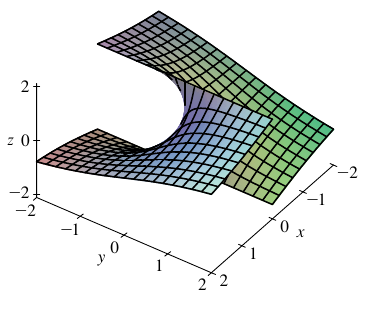
\includegraphics[scale=0.6]{figuras/cont1.png}
\end{center}
\end{frame}



\begin{frame}[label=limites]
	\frametitle{ }
	
		\uncover<1->{\begin{exe} Determine os pontos de continuidade de \begin{enumerate}[a]
					
					\item $f(x,y)=\left\{\begin{array}{ll}
						\dps\frac{2x^2y}{x^2+y^2}, &(x,y)\neq (0,0)\\
						\\
						0, & (x,y)=(0,0)\\
					\end{array}\right.$
					
					\item   $f(x,y)=\left\{\begin{array}{ll}
						\dps\frac{xy}{x^2+y^2}, &(x,y)\neq (0,0)\\
						\\
						0, & (x,y)=(0,0)\\
					\end{array}\right.$
				\end{enumerate}
		\end{exe} }
		
		\uncover<1->{Analogamente podemos generalizar estes resultados para funções de mais de duas variáveis quaisquer.}
		
\end{frame}

\begin{frame}[label=limites]
	\begin{casa}
		\begin{enumerate}
			\item Decida sobre a existência do seguinte limite $\dps\lim_{(x,y)\to(0,0)}\frac{x^2y}{x^4+y^2}$.
			
			\item Determine os pontos de continuidade da função
			\[f(x,y)=\begin{cases}
\frac{xy}{x^2+xy+y^2}, & (x,y)\neq (0,0),\\
0, & (x,y=(0,0).
			\end{cases}\]

\item Revise a definição de derivada de função de uma variável $y=f(x)$.
		\end{enumerate}
	\end{casa}
\end{frame}




